\documentclass[12pt]{article}

% --- Packages ---
\usepackage[utf8]{inputenc}
\usepackage[margin=1in]{geometry}
\usepackage{amsmath, amssymb, amsfonts, amsthm}
\usepackage{graphicx}
\usepackage{float}
\usepackage{hyperref}
\usepackage{enumerate}
\usepackage{mathpazo}
\usepackage{natbib}
\usepackage{tcolorbox}

% --- Document Information ---
\title{18-660 Optimization \\ Homework 1}
\author{\textbf{Name:} Edward Ajayi \\ \textbf{Andrew ID:} eaajayi \\ \textbf{Semester: }Spring 2026} % Enter your name here
\date{\textbf{Date: }\today}


\begin{document}

\maketitle
\newpage

\section*{Problem 1: Convex Functions}

\begin{enumerate}
    \item[(a)] \textbf{Function:} $f(x) = \frac{1}{x^2}$ over domain $(0, \infty)$.
    
    To determine the convexity, we examine the second derivative:
    $$ f(x) = x^{-2} \implies f'(x) = -2x^{-3} \implies f''(x) = 6x^{-4} = \frac{6}{x^4} $$
    Since the domain is $x > 0$, the term $x^4$ is always positive. Therefore, $f''(x) > 0$ for all $x \in (0, \infty)$, which satisfies the condition for \textbf{strict convexity}.
    
    However, the function is not strongly convex. As $x \to \infty$, $f''(x) \to 0$. Strong convexity requires $f''(x) \ge \mu$ for some constant $\mu > 0$ everywhere on the domain, which fails here as the curvature vanishes at infinity.
    
    \textbf{Answer: Strictly Convex}

    \item[(b)] \textbf{Function:} $f(x) = \min\{x, 1-x\}$ over domain $\mathbb{R}$.
    
    This function represents the pointwise minimum of two affine functions ($g(x)=x$ and $h(x)=1-x$). Affine functions are both convex and concave. 
    
    A known property of convexity is that the pointwise minimum of a set of concave functions is always concave. Geometrically, the graph forms an inverted "V" shape. Since the "legs" of the graph are linear (straight lines), it is not strictly concave.
    
    \textbf{Answer: Concave}

    \item[(c)] \textbf{Function:} $f(x) = (\theta^T x)_+ = \max\{0, \theta^T x\}$ over domain $\mathbb{R}^n$ (ReLU).
    
    This function is the pointwise maximum of two convex functions: the constant function $0$ and the linear function $\theta^T x$. The pointwise maximum of convex functions is always convex.
    
    It is not strictly convex because there exists a region (where $\theta^T x < 0$) where the function is identically zero (flat). In this region, the strict inequality definition of convexity ($\lambda f(x) + (1-\lambda)f(y) > f(\lambda x + (1-\lambda)y)$) does not hold, as the relationship becomes an equality.
    
    \textbf{Answer: Convex}

    % \item[(d)] \textbf{Function:} $f(x) = \text{sigm}(\theta^T x) = \frac{1}{1+e^{-\theta^T x}}$ over domain $\mathbb{R}^n$.
    
    % The sigmoid function $g(z) = \frac{1}{1+e^{-z}}$ changes curvature.
    % \begin{itemize}
    %     \item For $z < 0$, $g''(z) > 0$ (convex).
    %     \item For $z > 0$, $g''(z) < 0$ (concave).
    % \end{itemize}
    % Since the function exhibits both convex and concave behavior depending on the input region, it cannot be classified globally as either.
    
    % \textbf{Answer: Neither convex nor concave}

    \item[(d)] \textbf{Function:} $f(x) = \text{sigm}(\theta^T x) = \frac{1}{1+e^{-\theta^T x}}$ over domain $\mathbb{R}^n$.
    
    To classify the convexity, we define the scalar sigmoid function $g(z) = \frac{1}{1+e^{-z}}$, where $z = \theta^T x$. Since $\theta^T x$ is an affine transformation, the convexity of $f(x)$ depends entirely on the convexity of the scalar function $g(z)$. We analyze its second derivative:
    
    \begin{enumerate}
        \item \textbf{First Derivative:}
        The derivative of the sigmoid function satisfies the logistic differential equation:
        $$ g'(z) = \frac{e^{-z}}{(1+e^{-z})^2} = g(z)(1 - g(z)) $$
        Since $g(z) \in (0, 1)$, $g'(z)$ is strictly positive.
        
        \item \textbf{Second Derivative:}
        Differentiating again with respect to $z$:
        \begin{align*}
            g''(z) &= \frac{d}{dz} [g(z)(1 - g(z))] \\
                   &= g'(z)(1 - g(z)) + g(z)(-g'(z)) \\
                   &= g'(z)(1 - 2g(z))
        \end{align*}
        Substituting $g'(z)$ back into the equation:
        $$ g''(z) = g(z)(1 - g(z))(1 - 2g(z)) $$
    \end{enumerate}

    % \textbf{Analysis of Sign:}
    The sign of $g''(z)$ depends entirely on the term $(1 - 2g(z))$, as $g(z)$ and $g'(z)$ are always positive.
    \begin{itemize}
        \item \textbf{Case 1 ($z < 0$):} Here, $g(z) < 0.5$, which implies $2g(z) < 1$. Therefore, $g''(z) > 0$, meaning the function is locally \textbf{convex}.
        \item \textbf{Case 2 ($z > 0$):} Here, $g(z) > 0.5$, which implies $2g(z) > 1$. Therefore, $g''(z) < 0$, meaning the function is locally \textbf{concave}.
    \end{itemize}
    
    Since the function's Hessian is not positive semi-definite everywhere (nor negative semi-definite everywhere), it is globally neither convex nor concave.
    
    \textbf{Answer: Neither convex nor concave}
\end{enumerate}

\newpage
\section*{Problem 2: Convex Sets}

\subsection*{1. Properties of Convex Sets}

\begin{enumerate}
    \item[(a)] \textbf{Intersection of sets:} $S \cap T$ \\
    \textbf{Answer: Convex}
    
    \textbf{Proof:}
    Let $S$ and $T$ be convex sets. Let $x, y \in S \cap T$ be any two points in the intersection.
    By definition, this implies:
    $$ x \in S, y \in S \quad \text{and} \quad x \in T, y \in T $$
    Since $S$ is convex, the line segment $\theta x + (1-\theta)y$ lies entirely in $S$ for all $\theta \in [0,1]$.
    Since $T$ is convex, the same line segment lies entirely in $T$.
    Because the segment is in both $S$ and $T$, it must be in $S \cap T$. Thus, the intersection is convex.

    \item[(b)] \textbf{Union of sets:} $S \cup T$ \\
    \textbf{Answer: Not Convex}
    
    \textbf{Intuition:} 
    Convexity requires that you can travel in a straight line between \textit{any} two points in the set without leaving the set. If $S$ and $T$ are separated (disjoint) sets, drawing a line from a point in $S$ to a point in $T$ will cross the "empty space" between them. This empty space is not in the union, so convexity fails.
    
    \textbf{Counter-Example:}
    Let $S = \{0\}$ and $T = \{2\}$ in $\mathbb{R}$.
    The union is $S \cup T = \{0, 2\}$.
    Take $x=0$ and $y=2$. The midpoint is $z=1$.
    Since $1 \notin \{0, 2\}$, the set is not convex.

    \item[(c)] \textbf{Set difference:} $S \setminus T = \{x \mid x \in S, x \notin T\}$ \\
    \textbf{Answer: Not Convex}
    
    \textbf{Intuition:} 
    Imagine $S$ is a solid disk and $T$ is a smaller disk inside it. $S \setminus T$ creates a shape with a hole (like a donut). If you pick two points on opposite sides of the hole, the straight line connecting them passes through the hole. Since the hole (set $T$) has been removed, the line leaves the set $S \setminus T$, failing convexity.
    
    \textbf{Counter-Example:}
    Let $S = [-2, 2]$ and $T = (-1, 1)$. Both are convex intervals.
    The difference is $S \setminus T = [-2, -1] \cup [1, 2]$.
    Pick $x = -2$ and $y = 2$.
    The midpoint is $0$.
    Since $0 \in (-1, 1)$, $0$ is in $T$, which means $0 \notin S \setminus T$. Thus, the set is not convex.
\end{enumerate}

\subsection*{2. Examples}

\begin{enumerate}
    \item[(a)] \textbf{Set:} $S = \{x \in \mathbb{R}^n : \|x\|_2 \le 1\}$ \\
    \textbf{Answer: Convex}
    
    \textbf{Proof:}
    Let $x, y \in S$. This implies $\|x\|_2 \le 1$ and $\|y\|_2 \le 1$.
    Consider the point $z = \theta x + (1-\theta)y$ for $\theta \in [0,1]$.
    We use the triangle inequality and the homogeneity of the norm:
    $$ \|z\|_2 = \|\theta x + (1-\theta)y\|_2 \le \|\theta x\|_2 + \|(1-\theta)y\|_2 $$
    $$ \|z\|_2 \le \theta\|x\|_2 + (1-\theta)\|y\|_2 $$
    Substituting the bounds for $x$ and $y$:
    $$ \|z\|_2 \le \theta(1) + (1-\theta)(1) = 1 $$
    Thus $z \in S$, proving convexity.

    \item[(b)] \textbf{Set:} $S = \{x \mid x + B \subseteq A\}$ where $A$ is convex \\
    \textbf{Answer: Convex}
    
    \textbf{Proof:}
    The condition $x + B \subseteq A$ implies that for every element $b \in B$, the point $x+b$ must be in $A$.
    We can rewrite $S$ as an intersection of translated sets:
    $$ S = \bigcap_{b \in B} \{x \mid x + b \in A\} = \bigcap_{b \in B} (A - b) $$
    Since $A$ is convex, the translation $A-b$ is also convex (translation preserves geometry).
    From part 1(a), we proved that the intersection of convex sets is always convex. Therefore, $S$ is convex.

    \item[(c)] \textbf{Set:} Rank-constrained matrices $S = \{X \in \mathbb{S}^n \mid \text{rank}(X) = k\}$ \\
    \textbf{Answer: Not Convex}
    
    \textbf{Intuition:} 
    The rank of a sum of matrices is generally additive (or at least increases). If you take a matrix $X$ with rank $k$ and another matrix $Y$ with rank $k$ that "lives in a different subspace" (has different non-zero rows/cols), their average will often have rank $2k$ (or at least $>k$). Since the rank changes on the line segment, it doesn't stay equal to $k$.
    
    \textbf{Counter-Example:}
    Let $n=2, k=1$.
    Let $X = \begin{bmatrix} 1 & 0 \\ 0 & 0 \end{bmatrix}$ (Rank 1).
    Let $Y = \begin{bmatrix} -1 & 0 \\ 0 & 0 \end{bmatrix}$ (Rank 1).
    Consider the midpoint $Z = 0.5X + 0.5Y = \begin{bmatrix} 0 & 0 \\ 0 & 0 \end{bmatrix}$.
    The rank of $Z$ is 0, not 1. Thus $Z \notin S$.

    \item[(d)] \textbf{Set:} Sparsity constraint $S = \{x \in \mathbb{R}^n \mid \text{nnz}(x) \le k\}$ \\
    \textbf{Answer: Not Convex}
    
    \textbf{Intuition:} 
    This is similar to the rank problem. If you take a vector $x$ that has non-zeros in the first $k$ positions, and a vector $y$ that has non-zeros in the \textit{next} $k$ positions, they are both in the set $S$. However, their sum will have non-zeros in $2k$ positions. This sum is "less sparse" than the originals and falls outside the set.
    
    \textbf{Counter-Example:}
    Let $n=2, k=1$.
    Let $x = [1, 0]^\top$ (1 non-zero).
    Let $y = [0, 1]^\top$ (1 non-zero).
    The midpoint is $z = [0.5, 0.5]^\top$.
    This vector has 2 non-zero entries. Since $2 \not\le 1$, $z \notin S$.
\end{enumerate}

\newpage
\section*{Problem 3: Strong Convexity, Smoothness}

\subsection*{1. Monotonicity of Gradient}
\textbf{Proposition:} $f$ is convex if and only if $(\nabla f(x) - \nabla f(y))^T(x-y) \ge 0$.

\begin{proof}
\textbf{Direction $(\Rightarrow)$:} Assume $f$ is convex. By the first-order condition:
\begin{align}
    f(y) &\ge f(x) + \nabla f(x)^T(y-x) \\
    f(x) &\ge f(y) + \nabla f(y)^T(x-y)
\end{align}
Summing (1) and (2):
$$ f(y) + f(x) \ge f(x) + f(y) + \nabla f(x)^T(y-x) + \nabla f(y)^T(x-y) $$
$$ 0 \ge (\nabla f(x) - \nabla f(y))^T(y-x) + \nabla f(y)^T(y-y) $$
$$ (\nabla f(x) - \nabla f(y))^T(x-y) \ge 0 $$

\textbf{Direction $(\Leftarrow)$:} Assume monotonicity. Let $g(t) = f(x + t(y-x))$ for $t \in [0,1]$. By the fundamental theorem of calculus:
$$ f(y) - f(x) = g(1) - g(0) = \int_0^1 g'(t) dt = \int_0^1 \nabla f(x + t(y-x))^T (y-x) dt $$
We want to prove $f(y) \ge f(x) + \nabla f(x)^T(y-x)$. Subtract $\nabla f(x)^T(y-x)$ from both sides:
$$ f(y) - f(x) - \nabla f(x)^T(y-x) = \int_0^1 (\nabla f(x_t) - \nabla f(x))^T (y-x) dt $$
where $x_t = x+t(y-x)$. Note that $y-x = \frac{1}{t}(x_t - x)$. The integral integrand becomes:
$$ \frac{1}{t} (\nabla f(x_t) - \nabla f(x))^T (x_t - x) $$
By the monotonicity assumption, this term is $\ge 0$. Thus the integral is $\ge 0$, proving convexity.
\end{proof}

\subsection*{2. Smoothness Equivalence}
We prove the chain $(i) \implies (ii) \implies (iii) \implies (iv)$.

\textbf{(i) $\implies$ (ii):}
Given $\|\nabla f(x) - \nabla f(y)\| \le L\|x-y\|$. By Cauchy-Schwarz:
$$ (\nabla f(x) - \nabla f(y))^T(x-y) \le \|\nabla f(x) - \nabla f(y)\| \|x-y\| \le L\|x-y\|^2 $$

\textbf{(ii) $\implies$ (iii):}
Given $(\nabla f(x) - \nabla f(y))^T(x-y) \le L\|x-y\|^2$.
Let $y = x + tv$ for arbitrary $v$ and scalar $t$.
$$ (\nabla f(x+tv) - \nabla f(x))^T(tv) \le L\|tv\|^2 $$
Dividing by $t^2$ and taking $t \to 0$:
$$ v^T \nabla^2 f(x) v \le L\|v\|^2 = v^T (LI) v $$
Since this holds for all $v$, $\nabla^2 f(x) \preceq LI$.

\textbf{(iii) $\implies$ (iv):}
Given $\nabla^2 f(x) \preceq LI$. By Taylor's theorem with Lagrange remainder:
$$ f(y) = f(x) + \nabla f(x)^T(y-x) + \frac{1}{2}(y-x)^T \nabla^2 f(\xi) (y-x) $$
Since $\nabla^2 f(\xi) \preceq LI$, the quadratic term is bounded by $\frac{L}{2}\|y-x\|^2$.
$$ f(y) \le f(x) + \nabla f(x)^T(y-x) + \frac{L}{2}\|y-x\|^2 $$

\subsection*{3. Strong Convexity Equivalence}
We utilize the property that $f(x)$ is $\mu$-strongly convex iff $g(x) = f(x) - \frac{\mu}{2}\|x\|^2$ is convex.

\textbf{(i) $\iff$ (ii):}
Apply monotonicity of gradient to convex function $g(x)$:
$$ (\nabla g(x) - \nabla g(y))^T(x-y) \ge 0 $$
$$ (\nabla f(x) - \mu x - (\nabla f(y) - \mu y))^T(x-y) \ge 0 $$
$$ (\nabla f(x) - \nabla f(y))^T(x-y) - \mu\|x-y\|^2 \ge 0 \implies (\nabla f(x) - \nabla f(y))^T(x-y) \ge \mu\|x-y\|^2 $$

\textbf{(i) $\iff$ (iii):}
Apply Hessian condition to convex function $g(x)$:
$$ \nabla^2 g(x) \succeq 0 \implies \nabla^2 f(x) - \mu I \succeq 0 \implies \nabla^2 f(x) \succeq \mu I $$

\textbf{(i) $\iff$ (iv):}
Apply first-order condition to convex function $g(x)$:
$$ g(y) \ge g(x) + \nabla g(x)^T(y-x) $$
Substituting $g(x) = f(x) - \frac{\mu}{2}\|x\|^2$:
$$ f(y) - \frac{\mu}{2}\|y\|^2 \ge f(x) - \frac{\mu}{2}\|x\|^2 + (\nabla f(x) - \mu x)^T(y-x) $$
Rearranging yields:
$$ f(y) \ge f(x) + \nabla f(x)^T(y-x) + \frac{\mu}{2} \left( \|y\|^2 - \|x\|^2 - 2x^T(y-x) \right) $$
The term in parentheses simplifies to $\|y-x\|^2$, yielding:
$$ f(y) \ge f(x) + \nabla f(x)^T(y-x) + \frac{\mu}{2}\|y-x\|^2 $$

\newpage
\section*{Problem 4: Programming with CVX}

\subsection*{Part 1}

The resource allocation problem was solved using CVXPY with $n = 10$, $D = 10$, and $f_i(x_i) = -ix_i$.

\textbf{Results:}
\begin{itemize}
    \item Optimal value: $-100.0$
    \item Optimal allocation: $x_{10} = 10$, and $x_i = 0$ for $i = 1, \ldots, 9$
\end{itemize}

All resources are allocated to agent 10 because minimizing $\sum_{i} -ix_i$ is equivalent to maximizing $\sum_{i} ix_i$. Since this is a linear program, the optimum lies at a vertex of the feasible polytope, giving everything to the highest-valued agent.

\subsection*{Part 2}

Three values of the fairness parameter $\tau$ were tested:

\begin{table}[h]
\centering
\begin{tabular}{c|ccc}
\hline
$i$ & $\tau = 0.1$ & $\tau = 1.0$ & $\tau = 5.0$ \\
\hline
1  & 0.0111 & 0.1095 & 0.4531 \\
2  & 0.0125 & 0.1229 & 0.4982 \\
3  & 0.0143 & 0.1401 & 0.5533 \\
4  & 0.0166 & 0.1630 & 0.6222 \\
5  & 0.0200 & 0.1947 & 0.7107 \\
6  & 0.0249 & 0.2418 & 0.8284 \\
7  & 0.0332 & 0.3189 & 0.9927 \\
8  & 0.0497 & 0.4681 & 1.2388 \\
9  & 0.0990 & 0.8803 & 1.6468 \\
10 & 9.7187 & 7.3608 & 2.4559 \\
\hline
\textbf{Optimal Value} & $-95.97$ & $-80.18$ & $-62.96$ \\
\hline
\end{tabular}
\end{table}

\begin{figure}[H]
    \centering
    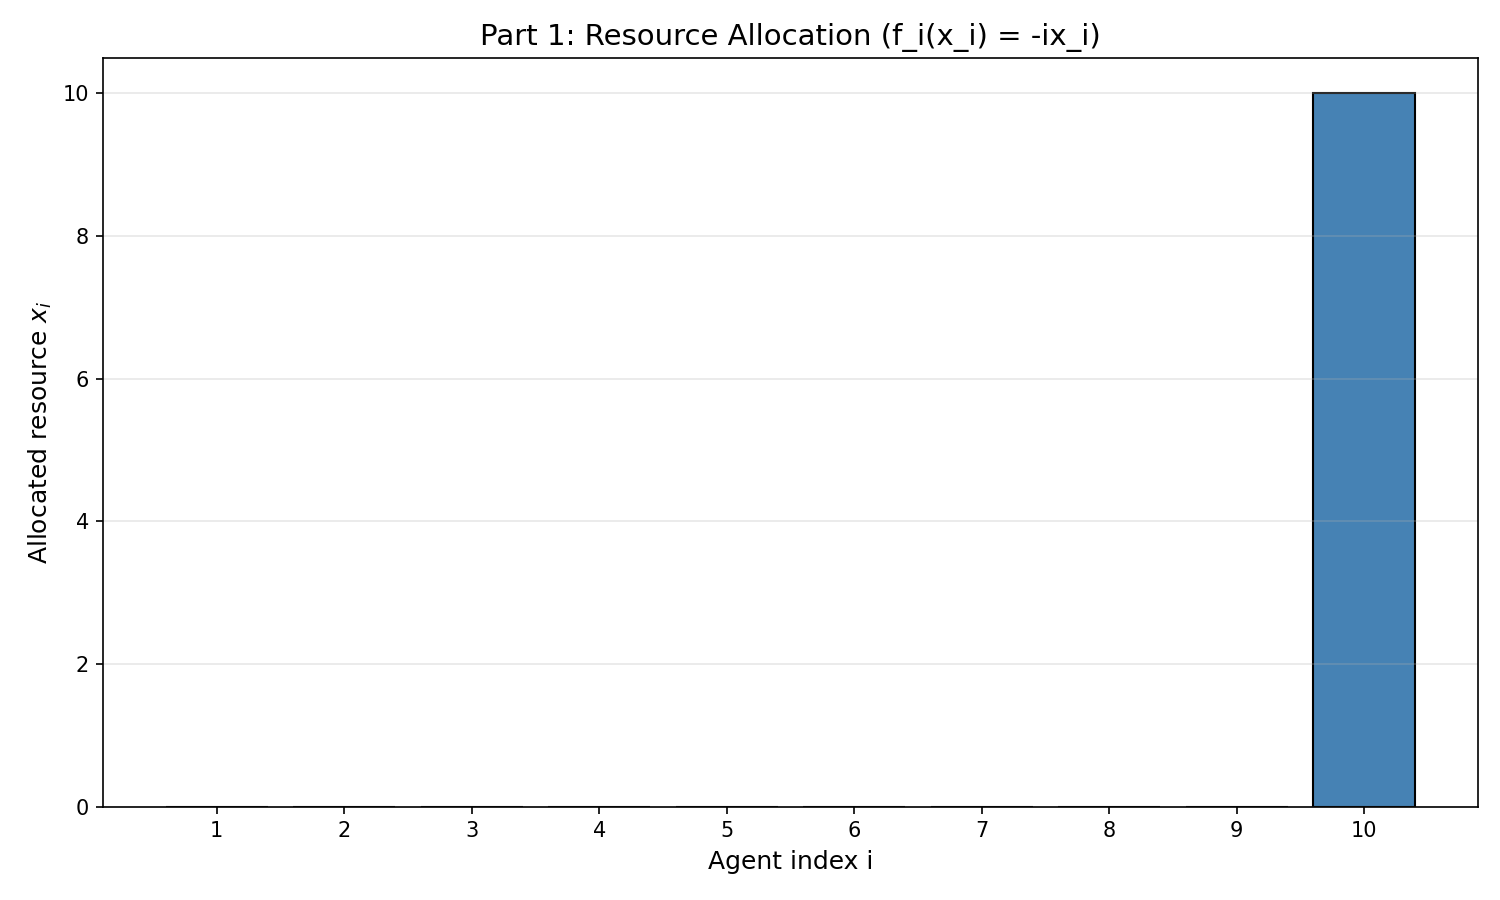
\includegraphics[width=0.8\textwidth]{problem4_part1.png}
    \caption{Resource allocation for Part 1 (no fairness constraints), showing concentration on agent 10.}
\end{figure}

\begin{figure}[H]
    \centering
    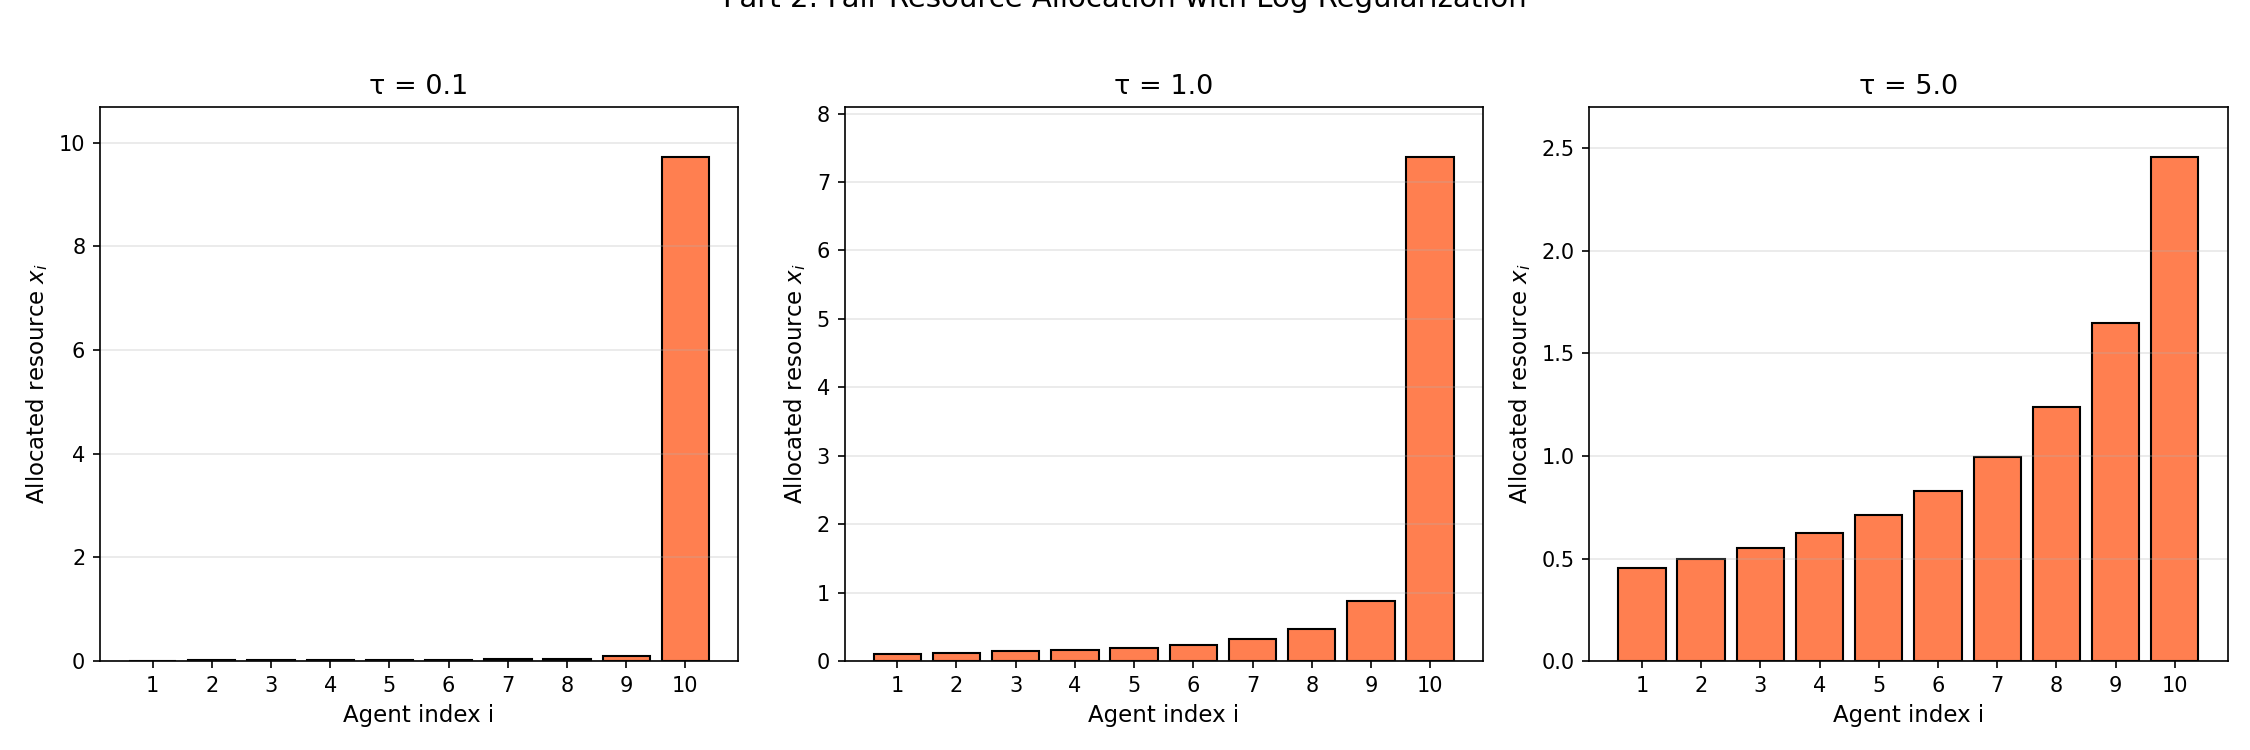
\includegraphics[width=\textwidth]{problem4_part2.png}
    \caption{Resource allocation for Part 2 for different values of $\tau$, demonstrating the impact of log regularization on fairness.}
\end{figure}

\begin{figure}[H]
    \centering
    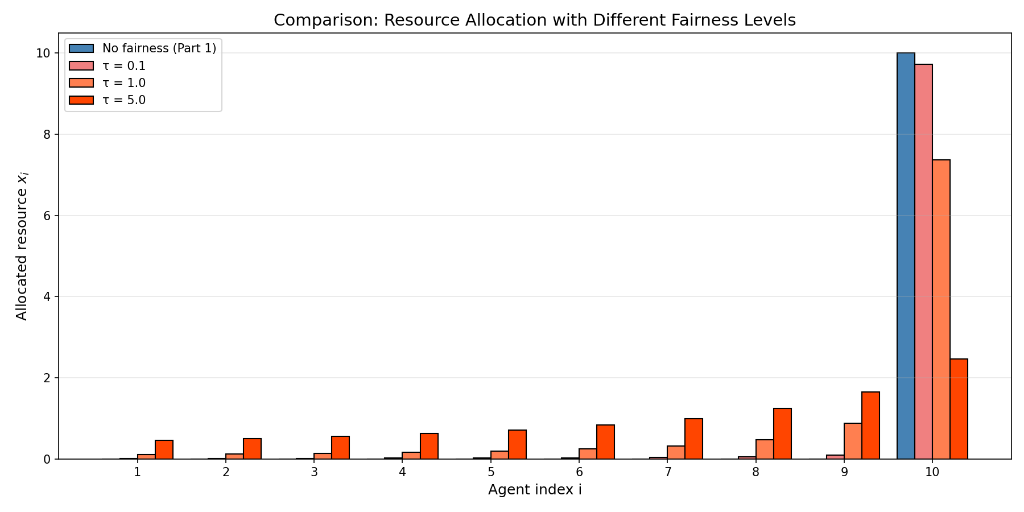
\includegraphics[width=\textwidth]{problem4_comparison.png}
    \caption{Comparison of resource allocations across all scenarios, highlighting the trade-off between individual agent utility and global allocation fairness.}
\end{figure}

\textbf{Observations:}
\begin{itemize}
    \item \textbf{$\tau = 0.1$:} Allocation is nearly identical to Part 1. Agent 10 receives 97.2\% of resources.
    \item \textbf{$\tau = 1.0$:} Resources spread more evenly. Agent 10 receives 73.6\%, but all agents get non-trivial allocations.
    \item \textbf{$\tau = 5.0$:} Distribution is much more uniform. Agent 10 receives only 24.6\%.
\end{itemize}

The log term promotes fairness because $\log(x) \to -\infty$ as $x \to 0^+$, creating an infinite penalty for giving any agent zero resources. Larger $\tau$ strengthens this fairness effect at the cost of lower utility (optimal value moves from $-100$ toward $-63$).


% ========== THE END ==========
\newpage
\section*{Declaration of External Resources}

Please fill out the following information with handwriting/typing and append this page to your homework submission.
\textbf{\emph{Failure to submit this declaration page will lead to a penalty on assignment credit.}}
You can use extra sheets of paper to answer the following questions if you need more space.

1. Have you collaborated with other students? If yes, name the collaborators and briefly describe the nature of collaboration.

Yes $\square$ \quad No $\boxtimes$

\begin{tcolorbox}
	% Your solution here
	\vspace{1in}
\end{tcolorbox}

2. Have you used GenAI in helping solve the problem? If yes, provide a brief description of how you used GenAI. You can also optionally append your chat history to your homework submission.

Yes $\square$ \quad No $\boxtimes$

\begin{tcolorbox}
	% Your solution here
	\vspace{1in}
\end{tcolorbox}

3. Cite all other external resources you used to finish the assignment.

\begin{tcolorbox}
	The following external resources were used to complete this assignment:
	\begin{enumerate}
		\item Boyd, S., and Vandenberghe, L. (2004). \textit{Convex Optimization}. Cambridge University Press.
		\item Rockafellar, R. T. (1970). \textit{Convex Analysis}. Princeton University Press.
		\item Diamond, S., and Boyd, S. (2016). CVXPY: A Python-Embedded Modeling Language for Convex Optimization. \textit{Journal of Machine Learning Research}, 17(83), 1-5.
	\end{enumerate}
\end{tcolorbox}

\end{document}